\chapter{Modern East Asia: Growth and Popular Culture}

\section{The ``East Asian miracle''}

From the 1950s to the 1990s, Japan, then the ``Four Little Dragons'' (South Korea, Taiwan,
Hong Kong, Singapore), then China grew faster for longer than any economies in history.

\begin{center}
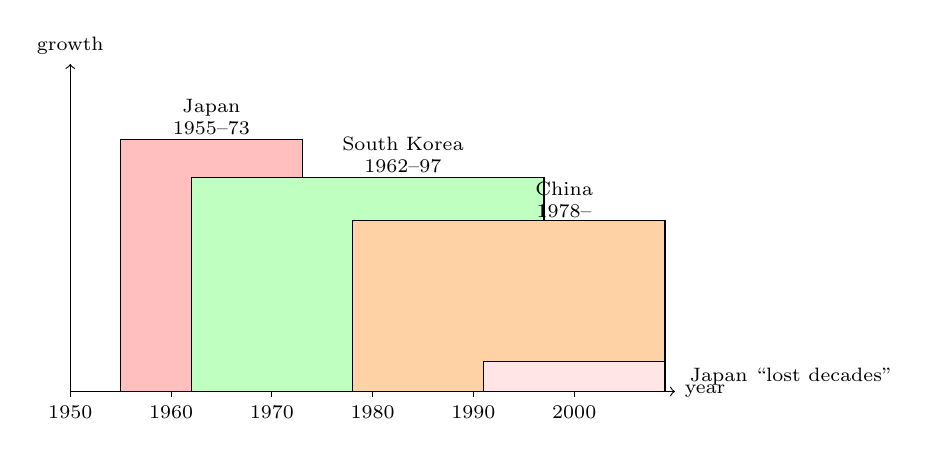
\begin{tikzpicture}[x=0.32cm, y=0.32cm, every node/.style={font=\scriptsize}]
  \draw[->] (0,0) -- (24,0) node[right] {year};
  \draw[->] (0,0) -- (0,13) node[above] {growth};
  \foreach \x/\l in {0/1950, 4/1960, 8/1970, 12/1980, 16/1990, 20/2000} {
    \draw (\x,0.2) -- (\x,-0.2) node[below] {\l};
  }
  % Japan high growth 1955-73
  \draw[fill=red!25] (2,0) rectangle (9.2,10) ;
  \node[align=center] at (5.6,10.9) {Japan\\1955--73};
  % Korea 1962-97
  \draw[fill=green!25] (4.8,0) rectangle (18.8,8.5);
  \node[align=center] at (13.2,9.4) {South Korea\\1962--97};
  % China from 1978
  \draw[fill=orange!35] (11.2,0) rectangle (23.6,6.8);
  \node[align=center] at (19.6,7.6) {China\\1978--};
  % Japan stagnation
  \draw[fill=red!10] (16.4,0) rectangle (23.6,1.2);
  \node[anchor=west] at (24.2,0.6) {Japan ``lost decades''};
\end{tikzpicture}
\end{center}

\begin{remark}
The figure is schematic (the heights only roughly indicate typical annual growth: about
10\% for Japan's high-growth era, 8\% for Korea, 9--10\% for China), but it shows the
``flying geese'' pattern: one economy after another took off, often moving into industries
the previous leader was leaving.
\end{remark}

\subsection{Japan}

\begin{itemize}
  \item \textbf{High-growth era} (1955--1973): average real growth near 10\% a year. The
        Ministry of International Trade and Industry (MITI) guided investment;
        \emph{keiretsu} business groups; lifetime employment and seniority wages in large
        firms; high savings; cheap US-provided security. By 1968 Japan was the
        second-largest capitalist economy.
  \item Symbols: the 1964 Tokyo Olympics and the \emph{shinkansen}; Sony, Toyota, Honda.
  \item \textbf{Bubble and burst}: a stock and real-estate bubble in the late 1980s collapsed
        in 1990--91, leading to the ``lost decade(s)'' of slow growth, deflation and an
        ageing, shrinking population.
\end{itemize}

\subsection{South Korea}

\begin{itemize}
  \item \textbf{Park Chung-hee} (military coup 1961, ruled until assassinated in 1979):
        export-oriented industrialization through five-year plans, state-directed credit to
        \emph{chaebol} (\ko{재벌}: Samsung, Hyundai, LG), heavy and chemical industry in the
        1970s. ``Miracle on the Han River.''
  \item Authoritarian rule: the Yushin constitution (1972), repression of labour and
        dissidents.
  \item \textbf{Democratization}: the Gwangju Uprising (May 1980) was brutally suppressed by
        Chun Doo-hwan's troops; mass protests in June 1987 forced direct presidential
        elections.
  \item The 1997 Asian Financial Crisis forced an IMF bailout; citizens donated gold to help
        repay it.
\end{itemize}

\subsection{China: reform and opening}

\begin{itemize}
  \item \textbf{Deng Xiaoping} (paramount leader from 1978): ``reform and opening''
        (\zh{改革开放}). Decollectivized agriculture (household responsibility system),
        Special Economic Zones (Shenzhen, 1980), foreign investment, gradual price reform.
  \item ``It doesn't matter whether a cat is black or white, as long as it catches mice.''
  \item \textbf{Tiananmen} (1989): student-led protests in Beijing ended with the army
        clearing the square on 4 June; economic reform continued, political reform did not.
  \item WTO entry (2001); ``workshop of the world''; second-largest economy by 2010.
\end{itemize}

\subsection{Explaining the miracle}

\begin{center}
\begin{tabular}{p{4cm}p{9cm}}
\toprule
Explanation & Argument \\
\midrule
Market / neoclassical & export orientation, macro stability, high savings and investment, education (World Bank, 1993) \\
Developmental state & a competent bureaucracy picked and disciplined industries (Chalmers Johnson on MITI; Alice Amsden on Korea) \\
Cultural (``Confucian'') & thrift, education, family and group loyalty; criticized as circular and as ignoring that the same culture was blamed for backwardness \\
Geopolitical & US aid, markets and security during the Cold War; colonial-era infrastructure (contested) \\
\bottomrule
\end{tabular}
\end{center}

\section{Popular culture: from consumers to exporters}

In the late 20th century East Asian popular culture became a major global export. The
course looked at two cases.

\subsection{Japan: anime, manga and ``Cool Japan''}

\begin{itemize}
  \item \textbf{Manga} (\ja{漫画}): Tezuka Osamu (\emph{Astro Boy}, 1952), the ``god of
        manga'', developed cinematic page layouts. Postwar weekly magazines (\emph{Shōnen
        Jump}, 1968) made manga a mass medium for all ages.
  \item \textbf{Anime} (\ja{アニメ}): TV anime from 1963 (\emph{Astro Boy}); \emph{Mobile
        Suit Gundam} (1979), \emph{Akira} (1988), Studio Ghibli (\emph{Spirited Away} won
        the 2003 Oscar), \emph{Pokémon} (1997).
  \item \textbf{Video games}: Nintendo, Sega, Sony PlayStation.
  \item The government's ``\textbf{Cool Japan}'' strategy (2010s) tried to turn this into
        soft power; Douglas McGray's 2002 article ``Japan's Gross National Cool'' coined the
        idea.
  \item Kawaii (\ja{かわいい}, ``cute'') culture: Hello Kitty (Sanrio, 1974).
\end{itemize}

\begin{aside}
Iwabuchi Kōichi called Japanese cultural exports ``culturally odourless'': anime characters
often do not look obviously Japanese, so products travel easily. The concept was debated in
tutorial: does Pokémon really have no ``odour'', or is its Japaneseness part of its appeal?
EASIA 120R takes this question much further.
\end{aside}

\subsection{Korea: Hallyu (the Korean Wave)}

\begin{definition}[Hallyu]
\emph{Hallyu} (\ko{한류}, \zht{韓流}, ``Korean current/wave'') is the term coined by Chinese
media in the late 1990s for the sudden popularity of South Korean TV dramas and pop music
in China and later across Asia and the world.
\end{definition}

\begin{center}
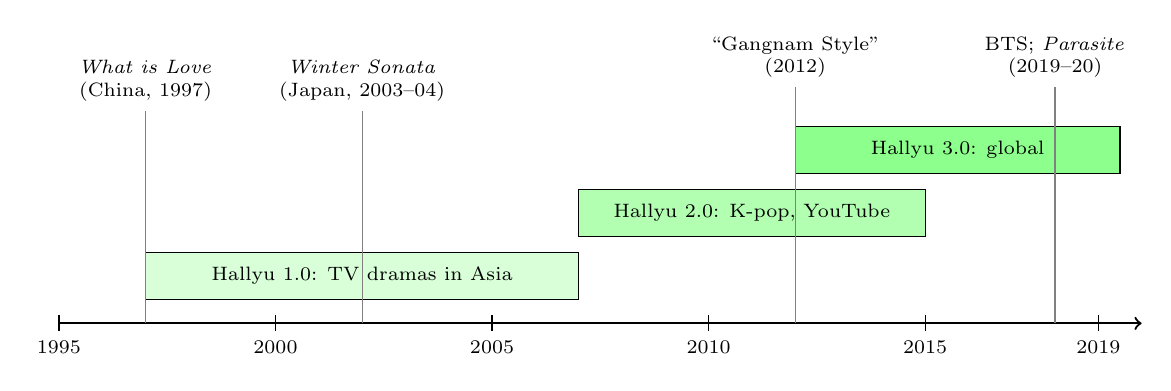
\begin{tikzpicture}[x=0.55cm, y=1cm, every node/.style={font=\scriptsize}]
  \draw[->, thick] (0,0) -- (25,0);
  \foreach \x/\l in {0/1995, 5/2000, 10/2005, 15/2010, 20/2015, 24/2019} {
    \draw (\x,0.1) -- (\x,-0.1) node[below] {\l};
  }
  \draw[fill=green!15] (2,0.3) rectangle (12,0.9) node[midway] {Hallyu 1.0: TV dramas in Asia};
  \draw[fill=green!30] (12,1.1) rectangle (20,1.7) node[midway] {Hallyu 2.0: K-pop, YouTube};
  \draw[fill=green!45] (17,1.9) rectangle (24.5,2.5) node[midway] {Hallyu 3.0: global};
  \foreach \x/\h/\l in {2/3.0/{\emph{What is Love}\\(China, 1997)}, 7/3.0/{\emph{Winter Sonata}\\(Japan, 2003--04)},
      17/3.3/{``Gangnam Style''\\(2012)}, 23/3.3/{BTS; \emph{Parasite}\\(2019--20)}} {
    \draw[gray] (\x,0) -- (\x,\h-0.3);
    \node[above, align=center] at (\x,\h-0.3) {\l};
  }
\end{tikzpicture}
\end{center}

\begin{itemize}
  \item \textbf{Causes}: the 1997 crisis pushed the government to promote cultural
        industries; deregulation of broadcasting; cheap high-quality dramas for Asian TV
        stations; idol-training systems of entertainment agencies (SM, YG, JYP); social
        media.
  \item \textbf{Winter Sonata} (\ko{겨울연가}) made actor Bae Yong-joon a star among middle-aged
        Japanese women and boosted tourism; it also complicated Japanese stereotypes of
        Korea.
  \item \textbf{K-pop}: idol groups, synchronized choreography, transnational fandoms.
  \item \textbf{Backlash}: anti-Hallyu protests in Japan (2011) and China's informal ban on
        Korean content after the THAAD missile dispute (2016).
\end{itemize}

\subsection{China}

China has been more a consumer than an exporter of popular culture, but its film industry
(Zhang Yimou, Jackie Chan in Hong Kong cinema, the 2008 Beijing Olympics ceremony),
platforms (WeChat, TikTok/Douyin) and online novels and dramas are growing. State
censorship shapes what can travel.

\section{Contemporary issues}

\begin{itemize}
  \item \textbf{Demography}: very low fertility (South Korea below 1.0 by 2018), rapid
        ageing; China's one-child policy (1980--2015).
  \item \textbf{Territorial disputes}: Senkaku/Diaoyu, Dokdo/Takeshima, the South China
        Sea.
  \item \textbf{History disputes}: comfort women, textbooks, Yasukuni (see Week 10).
  \item \textbf{North Korea}: nuclear tests from 2006; summits in 2018--19.
  \item \textbf{Hong Kong and Taiwan}: ``one country, two systems'' since 1997; Taiwan's
        democratic identity.
\end{itemize}

\section{Course conclusion}

\begin{center}
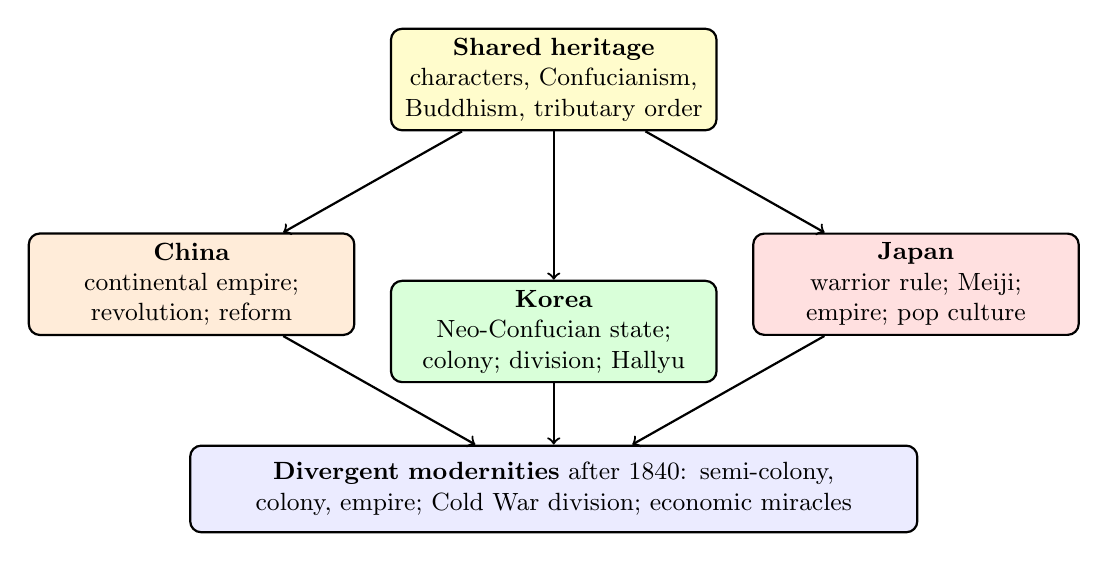
\begin{tikzpicture}[b/.style={draw, thick, rounded corners, align=center, font=\small, text width=3.9cm, minimum height=1.1cm}]
  \node[b, fill=yellow!20] (sh) at (0,2.6) {\textbf{Shared heritage}\\characters, Confucianism, Buddhism, tributary order};
  \node[b, fill=orange!15] (cn) at (-4.6,0) {\textbf{China}\\continental empire; revolution; reform};
  \node[b, fill=green!15] (kr) at (0,-0.6) {\textbf{Korea}\\Neo-Confucian state; colony; division; Hallyu};
  \node[b, fill=red!12] (jp) at (4.6,0) {\textbf{Japan}\\warrior rule; Meiji; empire; pop culture};
  \draw[->, thick] (sh) -- (cn); \draw[->, thick] (sh) -- (kr); \draw[->, thick] (sh) -- (jp);
  \node[b, fill=blue!8, text width=9cm] (mod) at (0,-2.6) {\textbf{Divergent modernities} after 1840: semi-colony, colony, empire; Cold War division; economic miracles};
  \draw[->, thick] (cn) -- (mod); \draw[->, thick] (kr) -- (mod); \draw[->, thick] (jp) -- (mod);
\end{tikzpicture}
\end{center}

\section*{Summary}
\begin{itemize}
  \item Japan (1955--73), the Four Dragons and China (from 1978) achieved sustained rapid
        growth; explanations range from markets to the developmental state to culture.
  \item South Korea and Taiwan democratized in 1987; China reformed its economy but not its
        politics.
  \item Anime/manga and Hallyu turned Japan and Korea into exporters of popular culture
        and soft power.
  \item The course's arc: shared heritage, local adaptation, divergent modernities.
\end{itemize}
